\documentclass[cal1spr16Lectures.tex]{subfiles}
%\AtBeginSubsection{
%	\begin{frame}[allowframebreaks]{}
%	\begin{multicols}{2}
%	\tableofcontents[currentsubsection]
%	\end{multicols}
%	\end{frame}
%	}
	
\begin{document}

%\section[Week 4]{Week 4: 8-12 February}

% % %
\subsubsection{\bf Wednesday 10 February}
\begin{frame}[allowframebreaks]{Wed 10 Feb}
\begin{itemize}\footnotesize
\item EXAM 1 on Friday.  
\begin{itemize}\footnotesize
	\item Covers up to \S 3.1 (see the semester schedule of material on the course webpage). 
	\item \alert{You must attend your own lecture on exam day.}  
	\item CEA: Register with the CEA office for a time on 12 Feb, as close to your normal lecture time as possible.
	\item Look at old Wheeler exams to study.
	\url{comp.uark.edu/~ashleykw}
	\item Also look at Quiz and Drill solutions posted in MLP.
	\item Do the book problems.  Go to office hours or Calculus Corner to get feedback.
\end{itemize}	
\framebreak
\item Quizzes: 
\begin{itemize}\footnotesize
	\item Include drill instructor and time.
	\item Don't turn in the Quiz sheet with your work.
	\item No quiz again until next week.
	\item Drill Exercise Tues 16 Feb and Quiz 4 Thurs 18 Feb.
\end{itemize}
\framebreak
\item  Announcement: 

\alert{A student in this class requires a note-taker. If you are willing to upload your notes and plan to attend class on a REGULAR basis, please sign up via the CEA Online Services on the Center for Educational Access (CEA) website \url{http://cea.uark.edu}. On the CEA Online Services login screen, click on ``Sign Up as a Note-taker". At the end of the semester you will receive verification of 48 community service hours OR a \$50 gift card for providing class notes. All interested students are encouraged to sign up; preference may be given to volunteers seeking community service in an effort engage U of A students in community service opportunities. Please contact the Center for Educational Access at ceanotes@uark.edu if you have any questions.}

\end{itemize}
\end{frame}

% % %
\begin{frame}
\begin{que}
Do the words ``derive" and ``differentiate" mean the same thing?
\end{que}
\end{frame}

% % %
\subsubsection{Graphing the Derivative}
% % %

% % %
\begin{frame}{\small Graphing the Derivative}
The graph of the derivative is the graph of the collection of slopes of tangent lines of a graph.  If you just have a graph (without an equation for the graph), the best you can do is approximate the graph of the derivative.
\end{frame}

% % %
\begin{frame}\footnotesize
\begin{ex}
\vspace{0.75pc}
\begin{columns}[T]
\begin{column}{0.45\textwidth}
	Simple checklist:
	\begin{itemize}
	\item[1.] Note where $f^{\prime}(x)=0$.
	\item[2.]  Note where $f^{\prime}(x)>0$.  (What does this look like?)
	\item[3.]  Note where $f^{\prime}(x)<0$.  (What does this look like?)
	\end{itemize}
\end{column}
\begin{column}{0.5\textwidth}	
	\centering{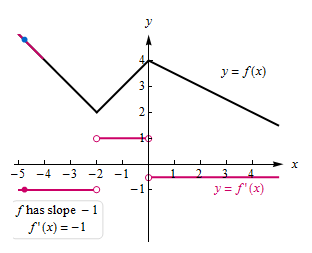
\includegraphics[scale=0.63]{pictures/graphDeriv3_1}}
\end{column}
\end{columns}
\end{ex}	
\end{frame}

% % %
\subsubsection{Differentiability vs. Continuity}
% % %

% % %
\begin{frame}{\small Differentiability vs. Continuity}
Key points about the relationship between differentiability and continuity:
\begin{itemize}
\item If $f$ is differentiable at $a$, then $f$ is continuous at $a$.
\item If $f$ is not continuous at $a$, then $f$ is not differentiable at $a$.
\item $f$ can be continuous at $a$, but not differentiable at $a$.
\end{itemize}
\end{frame}

% % %
\begin{frame}{}
A function $f$ is \alert{not} differentiable at $a$ if at least one of the following conditions holds:
\begin{itemize}
\item[1.] $f$ is not continuous at $a$.
\item[2.] $f$ has a corner at $a$.  
\begin{que} Why does this make $f$ not differentiable? \end{que}
\item[3.] $f$ has a vertical tangent at $a$.  
\begin{que} Why does this make $f$ not differentiable? \end{que}
\end{itemize}
\end{frame}

% % %
\subsubsection{Book Problems}
% % %

% % %
\begin{frame}
\begin{block}{3.1 Book Problems} 9-45 (odds), 49-53 (odds) \end{block}
\begin{itemize}
\item {\bf NOTE:}  You do not know any rules for differentiation yet (e.g., Power Rule, Chain Rule, etc.)  In this section, you are strictly using the definition of the derivative and the definition of slope of tangent lines we have derived.
\end{itemize}
\end{frame}


% % %
\subsection{Exam \#1 Review}
% % %

% % %
\begin{frame}[allowframebreaks]{Exam \#1 Review}\footnotesize
\begin{itemize}
\item \S 2.1  The Idea of Limits
	\begin{itemize}\footnotesize
	\item Understand the relationship between average velocity \& instantaneous velocity, and secant and tangent lines
	\item Be able to compute average velocities and use the idea of a limit to approximate instantaneous velocities
	\item Be able to compute slopes of secant lines and use the idea of a limit to approximate the slope of the tangent line
	\end{itemize}
\item \S 2.2 Definitions of Limits
	\begin{itemize}\footnotesize
	\item Know the definition of a limit
	\item Be able to use a graph of a table to determine a limit
	\item Know the relationship between one- and two-sided limits
	\end{itemize}
\framebreak	
\item \S 2.3 Techniques for Computing Limits
	\begin{itemize}\footnotesize
	\item Know and be able to compute limits using analytical methods (e.g., limit laws, additional techniques)
	\item Know the Squeeze Theorem and be able to use it to determine limits
	\end{itemize}
\begin{ex} Evaluate $\displaystyle\lim_{x\to 0}x\sin{\frac{1}{x}}$. \end{ex}	
\framebreak
\item \S 2.4 Infinite Limits
	\begin{itemize}\footnotesize
	\item Be able to use a graph, a table, or analytical methods to determine infinite limits
	\item Know the definition of a vertical asymptote  and be able to determine whether a function has vertical asymptotes 
	\end{itemize}
%\framebreak
\item \S 2.5 Limits at Infinity
	\begin{itemize}\footnotesize
	\item Be able to find limits at infinity and horizontal asymptotes 
	\item Know how to compute the limits at infinity of rational functions
	\end{itemize}
\framebreak	
\begin{ex} Determine the end behavior of $f(x)$.  If there is a horizontal asymptote, then say so.  Next, identify any vertical asymptotes.  If $x=a$ is a vertical asymptote, then evaluate $\displaystyle\lim_{x\to a^+}f(x)$ and $\displaystyle\lim_{x\to a^-}f(x)$.
\[f(x)=\frac{2x^3+10x^2+12x}{x^3+2x^2}\]
\end{ex}
\framebreak
\item \S 2.6 Continuity 
	\begin{itemize}\footnotesize
	\item Know the definition of continuity and be able to apply the continuity checklist
	\item Be able to determine the continuity of a function (including those with roots) on an interval
	\item Be able to apply the Intermediate Value Theorem to a function
	\end{itemize}
\framebreak
\begin{ex} Determine the value for $a$ that will make $f(x)$ continuous. 
\[f(x)=\begin{cases}
	\frac{x^2+3x+2}{x+1} & x\neq -1 \\
	a & x=-1
	\end{cases}\]
\end{ex}
\begin{ex} Show that $f(x)=2$ has a solution on the interval $(-1,1)$, with
\[f(x)=2x^3+x.\]
\end{ex}
\framebreak
\begin{exe}
What value of $k$ makes
\[
f(x)=\begin{cases}\frac{\sqrt{2x-5}-\sqrt{x+7}}{x-2} & x\neq 2 \\
	k & x=2
	\end{cases}
\]
continuous everywhere?
\end{exe}
\item $\oint$2.7 Precise Definition of Limits 
	\begin{itemize}\footnotesize
	\item Understand the $\delta$, $\epsilon$ relationship for limits
	\item Be able to use a graph or analytical methods to find a value for $\delta>0$ given an $\epsilon>0$ (including finding symmetric intervals)
	\end{itemize}
\framebreak
\begin{ex}
\vspace{0.75pc}
\begin{columns}[T]
	\begin{column}{.25\textwidth}
	\centering{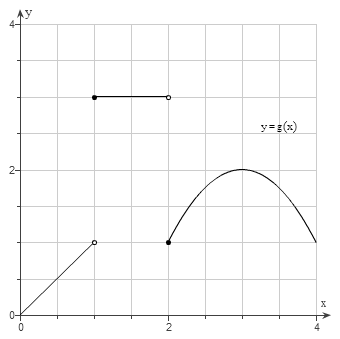
\includegraphics[scale=0.4]{pictures/Exam1pic}}
	\end{column}
	\begin{column}{.55\textwidth}
	Use the graph to find the appropriate $\delta$.
	\begin{itemize}\footnotesize
	\item[(a)]$|g(x)-2|<\textstyle\frac{1}{2}$ whenever 
	
	\hspace{6pc}$0<|x-3|<\delta$
	\item[(b)]$|g(x)-1|<\textstyle\frac{3}{2}$ whenever 
	
	\hspace{6pc}$0<|x-2|<\delta$
	\end{itemize}
	\end{column}
\end{columns}
\end{ex}
In this example, the two-sided limits at $x=1$ and $x=2$ do not exist.
\framebreak
\item \S 3.1 Introducing the Derivative
	\begin{itemize}\footnotesize
	\item Know the definition of a derivative and be able to use this definition to calculate the derivative of a given function
	\item Be able to determine the equation of a line tangent to the graph of a function at a given point
	\item Know the 3 conditions for when a function is not differentiable at a point, and why these three conditions make a function not differentiable at the given point
	\end{itemize}
\begin{ex}
	\begin{itemize}\footnotesize
	\item[(a)] Use the limit definition of the derivative to find an equation for the line tangent to $f(x)$ at $a$, where
	\[f(x)=\frac{1}{x};\quad a=-5.\]
	\item[(b)] Using the same $f(x)$ from part (a), find a formula for $f'(x)$ (using the limit definition).
	\item[(c)] Plug $-5$ into your answer for (b) and make sure it matches your answer for (a).
	\end{itemize}
\end{ex}
\end{itemize}
\end{frame}

% % %
\subsubsection{Other Study Tips}
% % %

% % %
\begin{frame}{\small Other Study Tips}\footnotesize
\begin{itemize}
\item Brush up on algebra, especially radicals.
%\item If your answer is something like $\sqrt 2$, don't plug that into your calculator, just leave it as is.
\item When in doubt, show steps.  Defer to class notes and old exams to get an idea of what's expected.
\item You will be punished for wrong notation; e.g., the limit symbol.
\item Read the question!  Several students always lose points because they didn't answer the question or they didn't follow directions.
\item Do the book problems.
%\item Look at the pictures in the book and the interactive applets on MLP.
\item Budget your time.  You don't have to do the problems in order.  Do the easier ones first.
\end{itemize}
\end{frame}

\end{document}